\begin{figure}[H]
    \begin{subfigure}[t]{.5\textwidth}
        \caption{}
        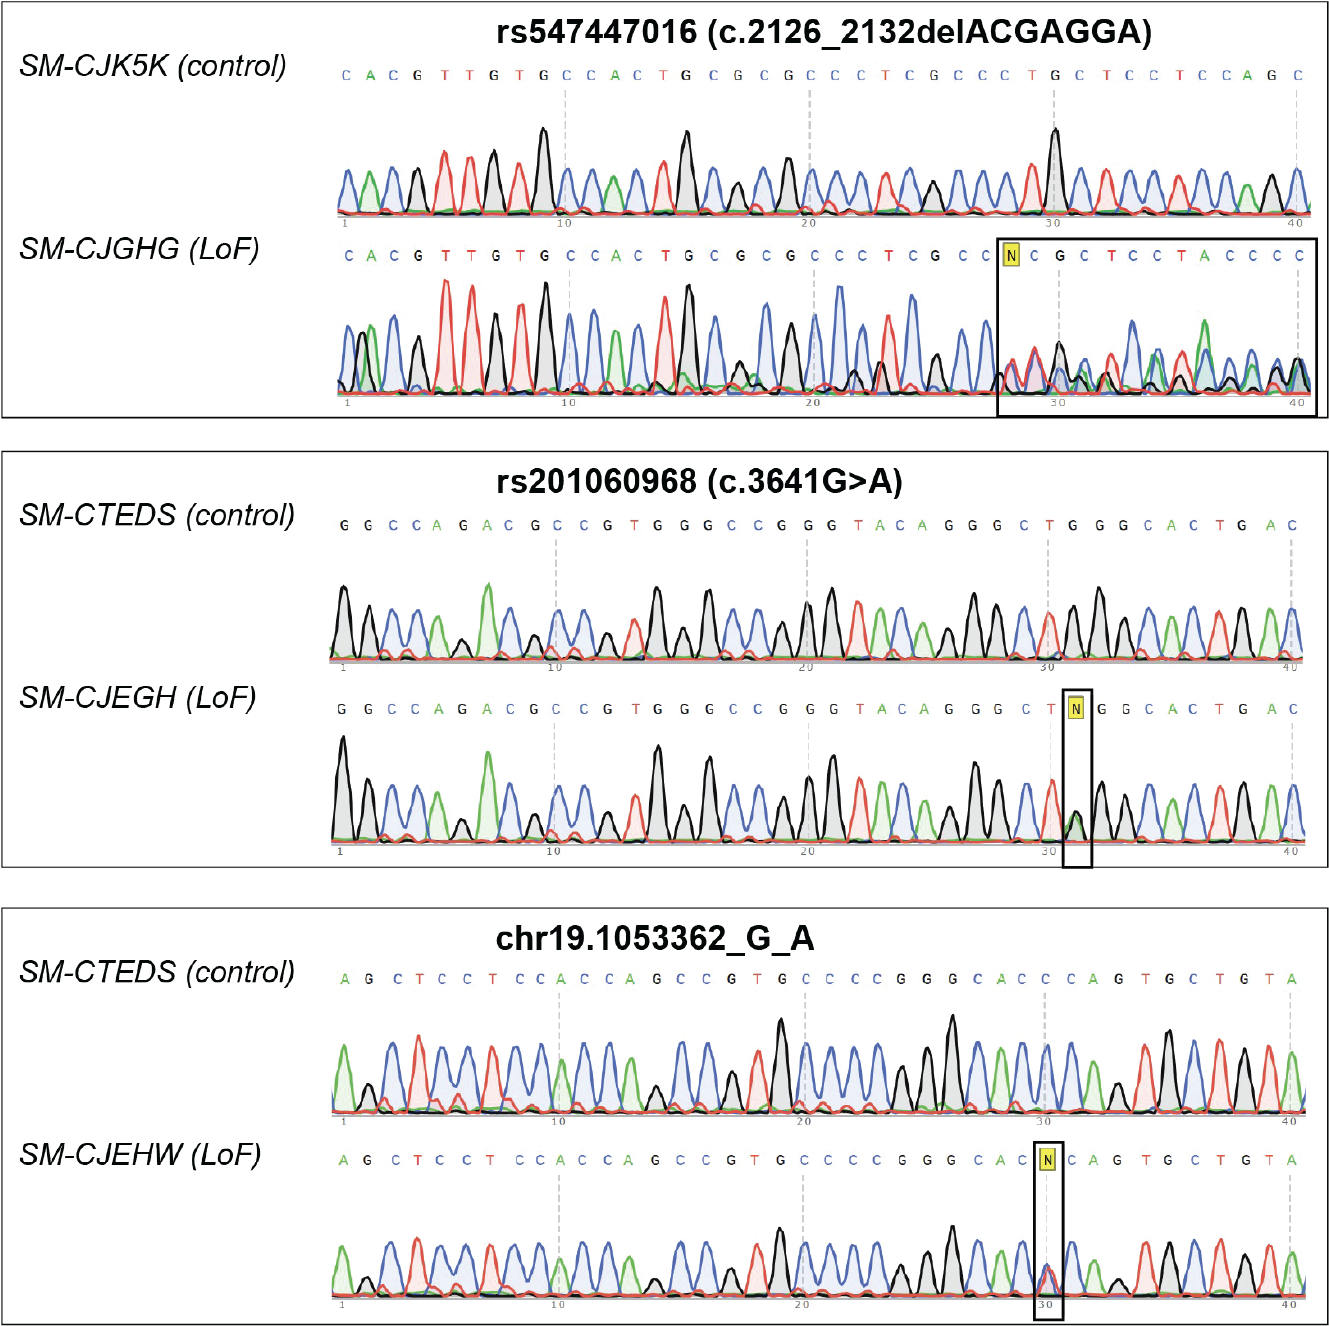
\includegraphics[width=\textwidth]{./extended_plots/sanger_seq.png}        
    \end{subfigure}  
    \begin{subfigure}[t]{.5\textwidth}
        \begin{subfigure}[t]{\textwidth}
            \caption{}
            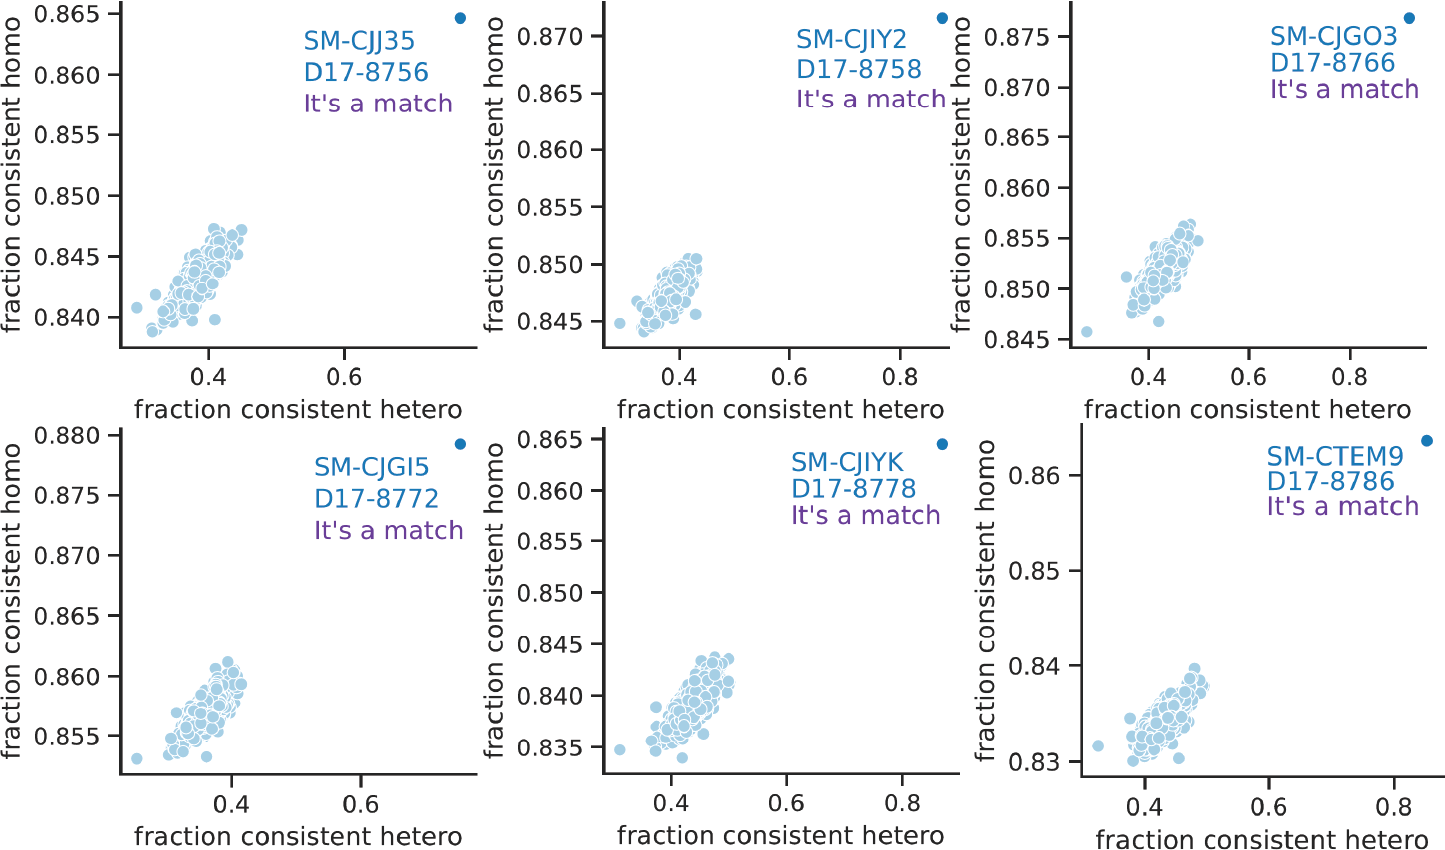
\includegraphics[width=\textwidth]{./extended_plots/sample_swap.png}        
        \end{subfigure}  
        \begin{subfigure}[t]{\textwidth}
            \caption{}
            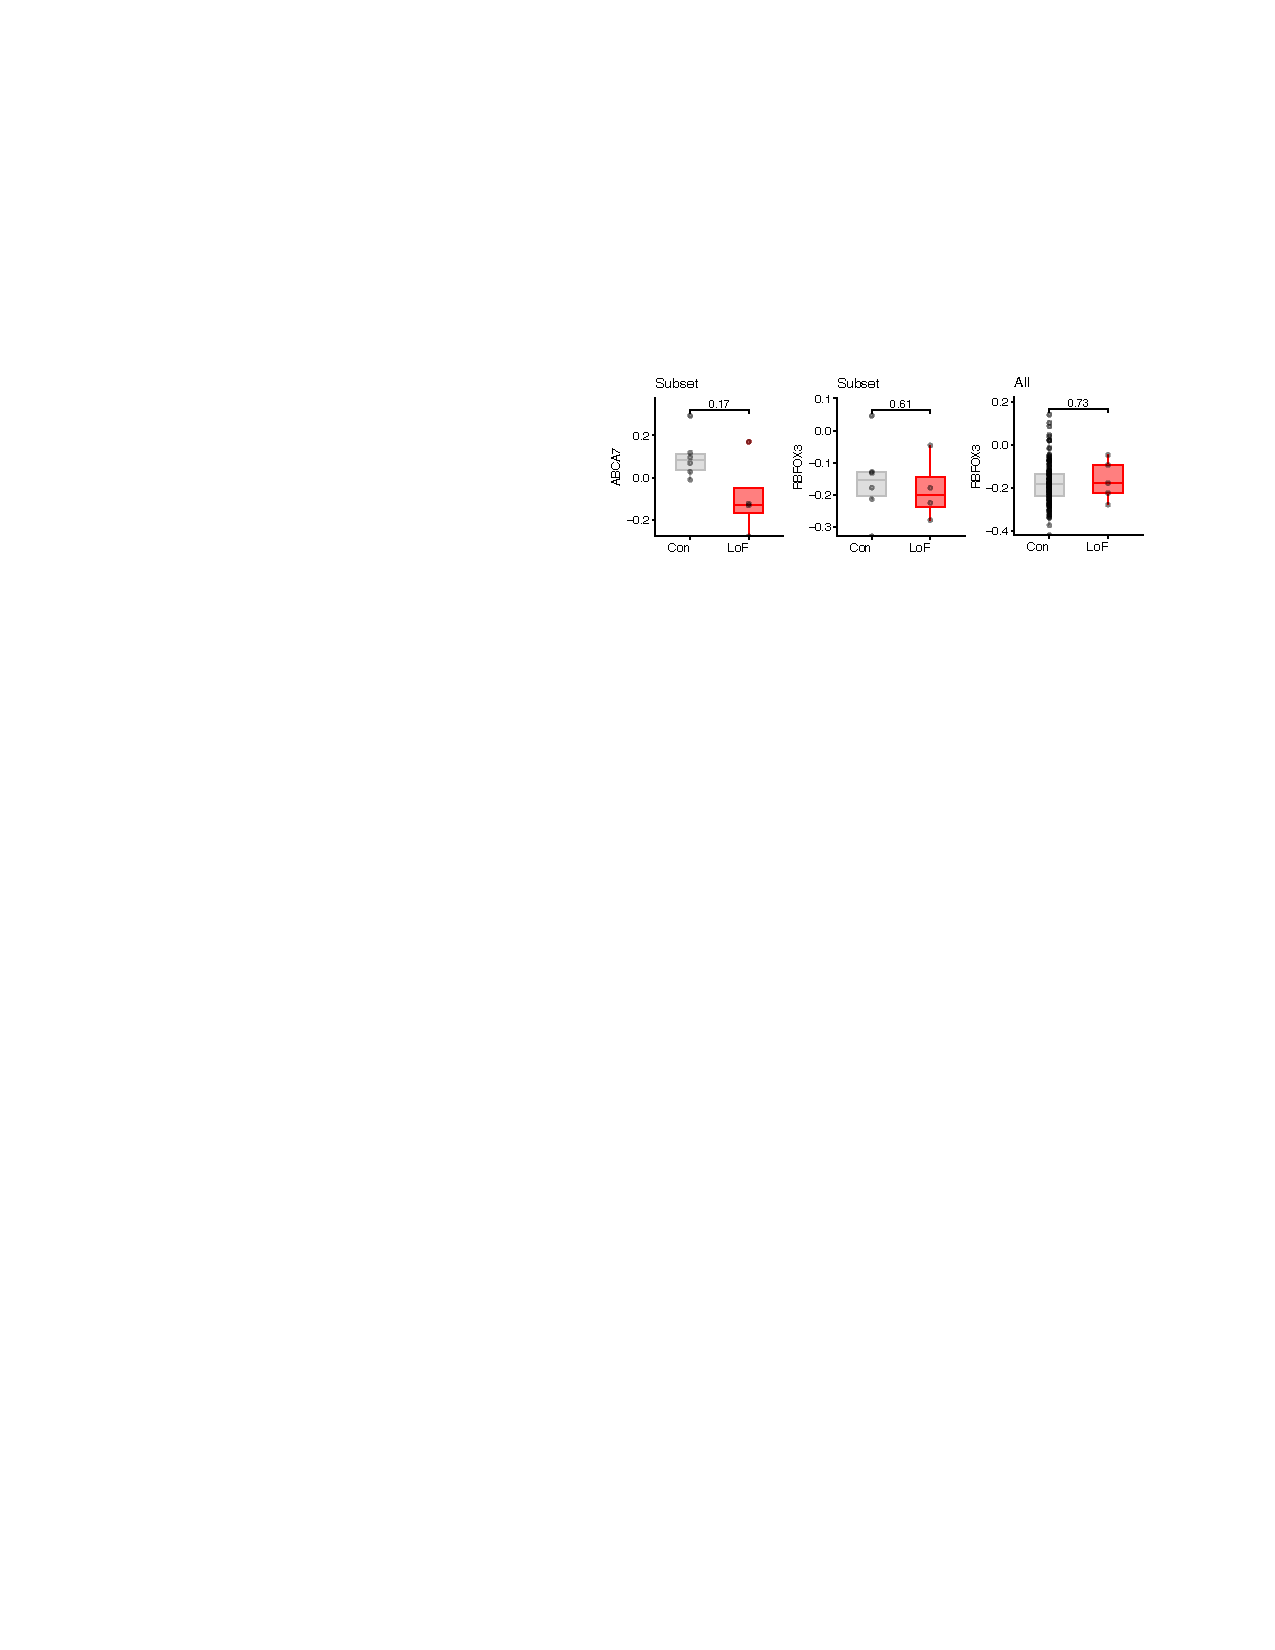
\includegraphics[width=\textwidth]{./extended_plots/protein_levels_extended.pdf}        
        \end{subfigure}  
    \end{subfigure}  
    \begin{subfigure}[t]{\textwidth}
        \caption{}
        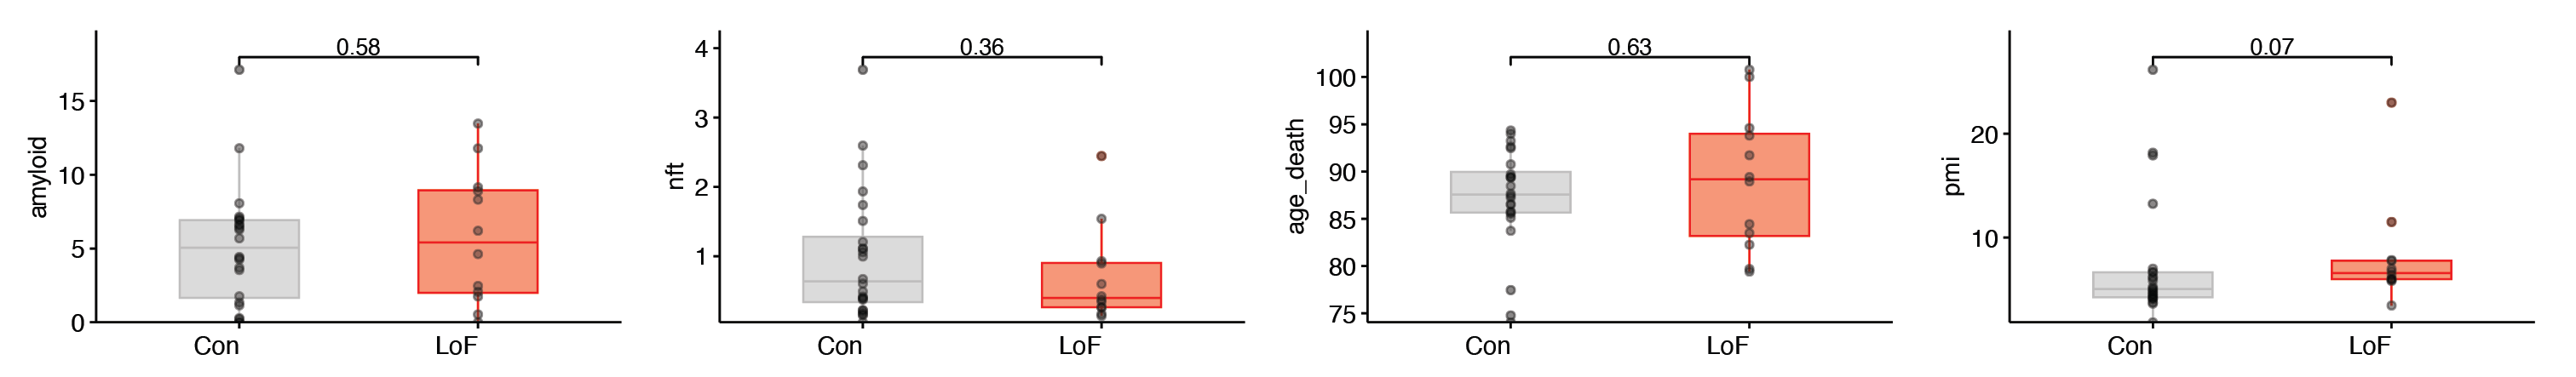
\includegraphics[width=\textwidth]{./extended_plots/batch_cont_var.png}        
    \end{subfigure}  
    \begin{subfigure}[t]{\textwidth}
        \caption{}
        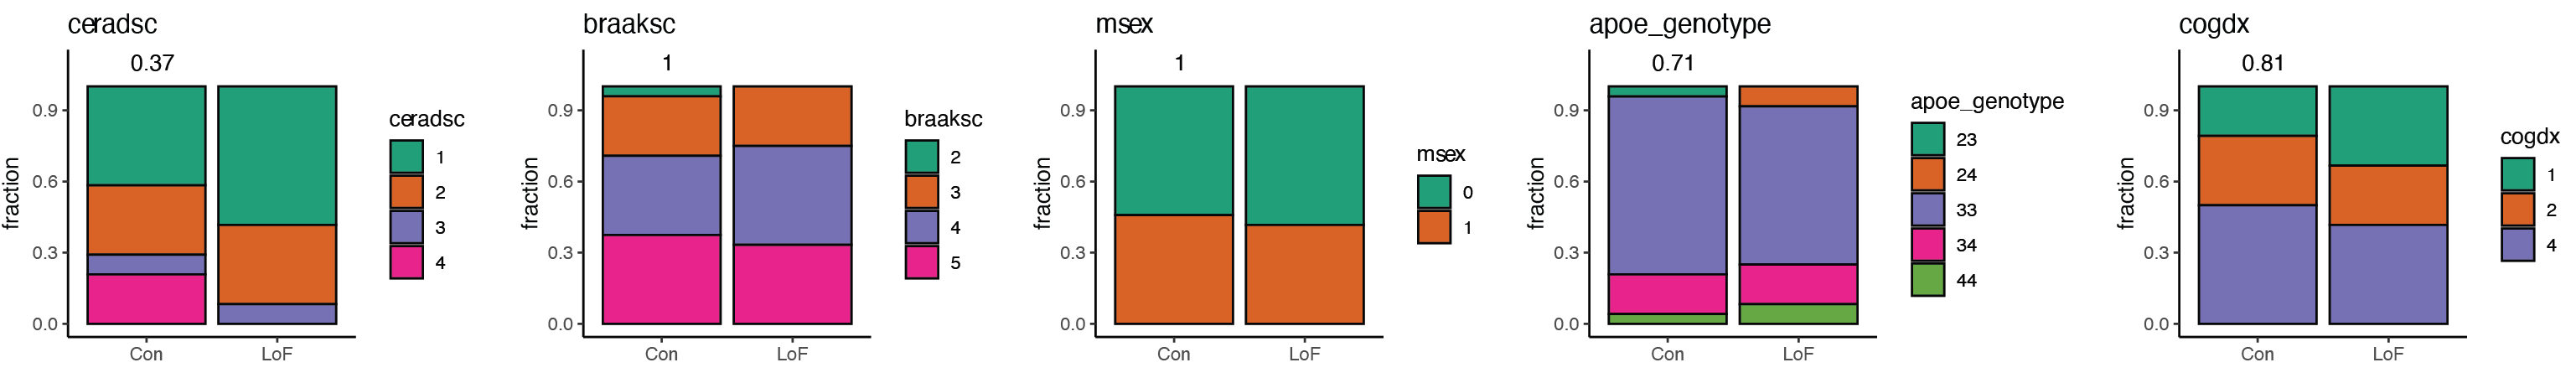
\includegraphics[width=\textwidth]{./extended_plots/batch_categorical_vars.png}        
    \end{subfigure}  
    \caption{
        \textbf{Overview of Human snRNA-Sequencing Cohort.}\\
    }
    \label{fig:snRNA_cohort}
\end{figure}
\begin{itemize}
    \item[\textbf{(A)}] Sanger sequencing of ABCA7 LoF variants in prefrontal cortex genomic DNA samples from 3 ABCA7 LoF carriers and 3 controls from the snRNA-seq cohort. Sequencing confirmed heterozygosity of the indicated variant in LoF samples, with variant location marked by a black box. 
    \item[\textbf{(B)}] Example plots validating matches between whole genome sequencing (WGS) and snRNA-seq libraries. Each plot shows the concordance of homo- and heterozygous SNP calls between WGS and snRNA-seq data for a single individual. Matches between WGS SNP calls and snRNA-seq BAM inferred SNP calls are indicated by extreme outliers. Expected (i.e., correct) matches are indicated in blue/purple. 
    \item[\textbf{(C)}] Protein levels from post-mortem human prefrontal cortex (see Table~\ref{tab:external_datasets} for external dataset used) showing ABCA7 protein levels (left) and NeuN (RBFOX3) levels (middle) for a subset of individuals in the snRNA-seq cohort (N=6 control and N=4 ABCA7 LoF carriers). The right panel shows NeuN (RBFOX3) protein levels by genotype in all available control samples (N=180) vs. ABCA7 LoF carriers (N=5). 
    \item[\textbf{(D)}] Distributions of continuous metadata variables (see Supplementary Text for descriptions) for control individuals (N=24) vs. ABCA7 LoF carriers (N=12). For panels C and D, boxes indicate dataset quartiles per condition, and whiskers extend to the most extreme data points not considered outliers (i.e., within 1.5 times the interquartile range from the first or third quartile). 
    \item[\textbf{(E)}] Distributions of discrete metadata variables for control individuals (N=24) vs. ABCA7 LoF carriers (N=12). Con=control, LoF=ABCA7 loss-of-function. P-values in panels C and D were computed by two-sided Wilcoxon rank sum test. P-values in panel E were computed by two-sided Fisher’s exact test.
\end{itemize}